\documentclass[accentcolor=tud9c,colorbacktitle,inverttitle,landscape,german,presentation,t]{tudbeamer}
\usepackage{amstext}
\usepackage{amsmath}
\usepackage{graphicx}
\usepackage{multicol}
\usepackage{mathtools}
\usepackage{subfigure}
\usepackage[ngerman,english]{babel}
\usepackage[utf8]{inputenc}
\usepackage{colortbl}
\usepackage{adjustbox}

\begin{document}

\title{\"Ubung 9 - Gruppe 142}
\subtitle{Visual Computing - 3D-Visualisierung}

\author[Johannes Beck, Christian Eilers, Robin Menzenbach, Martin Steinborn]{Johannes Beck, Christian Eilers, Robin Menzenbach, Martin Steinborn}


\date{\today}

\begin{titleframe}
\end{titleframe}

\section{Aufgabe 1}
	\begin{frame}
		\frametitle{Aufgabe 1: 3D-Daten}
		%TODO: Nennen und beschreiben Sie zwei Beispiele für die Anwendung von 3D-Daten, welche nicht in der Vorlesung vorgestellt wurden.
3D-Daten können nicht nur Gewonnen, sondern auch genutzt werden, um dinge dar- oder herzustellem. Beispiele hierfür wären 3D Drucker oder CAD Software.
		
	\end{frame}

\section{Aufgabe 2}
\begin{frame}
	\frametitle{Aufgabe 2: Volumenvisualisierung}
			\begin{itemize}
		\item[a)] %TODO: Betrachten Sie folgende zwei Bilder:[Abbildung1] [Abbildung2]. Geben Sie für diese an, bei welchem direkte und bei welchem indirekte Volumenvisualisierung verwendet wurde. Wie funktionieren jeweils die beiden Methoden?
		
		\item[b)] %TODO: Wie können sehr große Oberflächennetze effektiv gerendert werden? Welche beiden Methoden werden dabei häufig angewendet und wieso?
	\end{itemize}
\end{frame}
\begin{frame}
	\frametitle{Aufgabe 2: Volumenvisualisierung}
	\begin{itemize}
		\item[c)] %Nennen Sie die drei in der Vorlesung vorgestellten Arten von Culling und beschreiben Sie sie!
			\begin{itemize}
				\item Backface-Culling: Polygone, bei denen lediglich die Rückseiten sichtbar sind (Polygonnormale zeigen vom Sichtpunkt werg), werden nicht gezeichnet. \\
				\item View-Frustum-Culling: PÜolygone, welche zum teil oder vollständig außerhalb des View-Frustums liegen werden nur zum Teil oder überhaupt nicht gezeichnet.\\
				\item Occlusion-Culling:Polygone werden nach Tiefe sortiert und nur gerendert wenn sie unter beachtung der Transparenz der überliegenden Polygone nicht vollständig verdeckt sind.\\
			\end{itemize}
		
		\item[d)] %TODO: Was wird bei der Polygon-Repräsentation von Isoflächen gemacht?
	\end{itemize}
\end{frame}

\section{Aufgabe 3}
\begin{frame}
	\frametitle{Aufgabe 3: Voronoi-Diagramme}
	\begin{itemize}
	\item[a)] %Wenden Sie die Delaunay-Triangulation grafisch auf das folgende Diagramm an.
	Die Delauney-Triaangulierung des angegebenen Diagramms ist in Abbildung \ref{DelTri} abgebildet. Wie man sehen kann enthält der Umkreis eines jeden Dreiecks lediglich die eigenen Punkte und keine Weiteren. Somit liegt eine korrekte Delauney-Triangulierung vor.
	\begin{figure}
		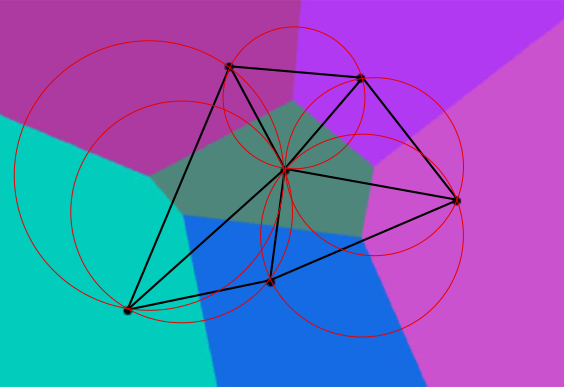
\includegraphics[width = .5\linewidth]{task_3a.png}
		\caption{Delauney-Triangulierung des gegebenen Diagramms}
		\label{DelTri}
	\end{figure}
	\end{itemize} 
\end{frame}
\begin{frame}
	\frametitle{Aufgabe 3: Voronoi-Diagramme}
	\begin{itemize}
	\item[b)] %Wann muss Edge-Flipping bei der Erstellung einer Delaunay-Triangulation durchgeführt werden? Wie funktioniert es und welche Eigenschaften haben die Dreiecke danach?
	Bei der Erstellung einer Delauney-Triangulierung muss Edge-Flipping angewendet werden, wenn der Umkreis eines Dreiecks einen Punkt eines anderen Dreiecks einschließt. Da dies nicht zulässig ist, wird die gemeinsame Kante der beiden Dreiecke gelöst und die beiden anderen Punkte verbunden. Diesen Vorgang nennt man Edge-Flipping. Ist lediglich eine Punktmenge als ausgangspunkt gegeben, kann diese zu beliebigen Dreiecken(ohne Kantenüberschneidung)  verbunden werden, welche dann mittels Edge-Flipping an Fehlerhaften Stellen in eine Delauney-Triangulierung überführt werden kann. 
	\end{itemize} 
\end{frame}

\section{Aufgabe 4}
\begin{frame}
	\frametitle{Aufgabe 4: Volume Rendering und Marching Cubes}
	\begin{itemize}
	\item[a)] %TODO: Beschreiben Sie die Faktoren, die die Laufzeit des jeweiligen Algorithmus maßgeblich beeinflussen.
		\begin{itemize}
			\item Marching-Cubes: \\
			\item Ray-Casting: 
		\end{itemize}
	\item[b)] %TODO: Nennen Sie einen Vor- und einen Nachteil von Volume Rendering gegenüber Marching Cubes.
	\begin{itemize}
		\item Vorteil: \\
		\item Nachteil: 
	\end{itemize}
	\end{itemize}
\end{frame}

\section{Aufgabe 5}
\begin{frame}
	\frametitle{Aufgabe 5: Marching Squares}
	\begin{itemize}
		\item[a)] %TODO: Was wird das Ergebnis der Anwendung der Marching Squares auf dieses Feld für einen gegeben	Isowert sein?
		
	\end{itemize}
\end{frame}
\begin{frame}
	\frametitle{Aufgabe 5: Marching Squares}
	\begin{itemize}
		\item[b)] %Wenden Sie den Marching Squares Algorithmus auf folgendes Feld an. Innerhalb der Isofläche sollen Werte liegen, die größer oder gleich 31 sind.
		Die Abbildung zeigt die Anwendung des Marching Squares Algorithmus mit Isowert auf das vorgegebene Feld. Die Werte innerhalb des Isofläche wurden grau hinterlegt, sowie die Umrandung in schwarz eingefügt.
		\begin{figure}
			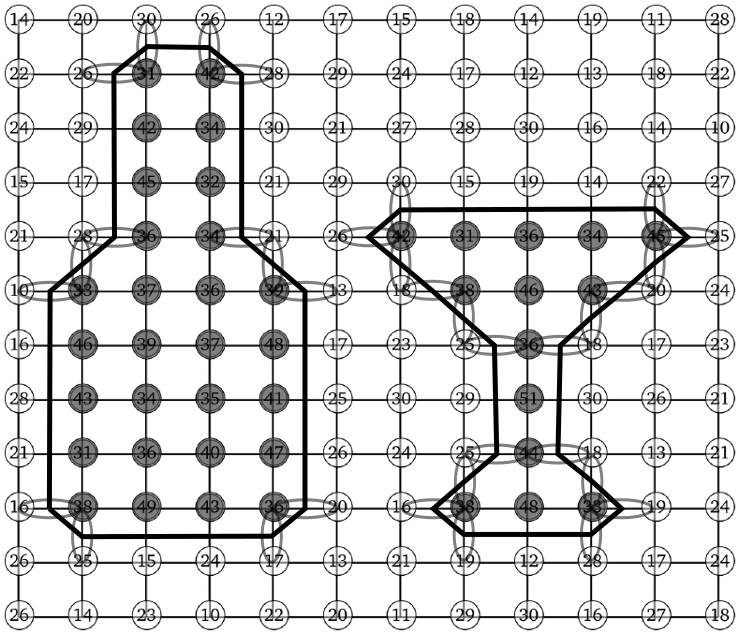
\includegraphics[width = .4\linewidth]{task_5b.png}
			\caption{Anwendung des Marching Squares Algorithmus uaf das gegebene Feld mit Isowert 31}
			\label{MaSq}
		\end{figure}
	\end{itemize}
\end{frame}
\end{document}
